
\documentclass[12pt]{article}
\usepackage{graphics,graphicx}
\usepackage{times,amsfonts,amssymb,latexsym,amsmath}
%\usepackage[citecolor=black]{hyperref}
\usepackage{url}
\usepackage[T1]{fontenc}              % T1 font encoding as default
%\usepackage[latin9]{inputenc}         % ISO-8859-15 (Latin 9) text
% ISO-8859-15 check: you should see both the euro and cent signs here:
% (if not, you are using a font that is not Latin 9 compatible)

\usepackage[a4paper]{geometry}        % DIN A4 paper
\geometry{lmargin=3cm, rmargin=3cm,tmargin=3cm, bmargin=3cm}

\usepackage{amsmath,amssymb}          % AMS TeX support
                 % Times font
\usepackage{bm}                       % bold math
\usepackage{tabularx}

\sloppy                               % don't be fussy in paragraph

\usepackage{url}                      % URL command
\usepackage{xspace}                   % gentle spacing after a macro
\usepackage{color}
\usepackage{ulem}
\definecolor{gray}{rgb}{0.4,0.4,0.4}

\usepackage{graphicx}
%\usepackage{ngerman}
\usepackage{amsmath}
\usepackage{amssymb}
\usepackage{latexsym}
\usepackage[round]{natbib}
\usepackage{graphicx}
\usepackage{mathrsfs}
\usepackage{subcaption}
%\usepackage{dsfont}   %%% fuer \N, \R etc

%\usepackage{bbm}
\usepackage{setspace}

%\usepackage[square,numbers]{natbib}
%\bibliographystyle{unsrtnat}
\usepackage{natbib}
\bibliographystyle{elsart-harv}
            % line spacing
%\singlespacing
%\onehalfspacing
\doublespacing

%\newtheorem{lemma}{Lemma}
%\newtheorem{theorem}{Theorem}
%\newtheorem{proof}{\textit{Proof}}

\bmdefine\X{X}
\bmdefine\Z{Z}
\bmdefine\x{x}
\bmdefine\z{z}
\bmdefine\y{y}
\bmdefine\Y{Y}

\bmdefine\M{M}
\bmdefine\Q{Q}
\bmdefine\P{P}
\bmdefine\w{w}
\bmdefine\W{W}
\bmdefine\p{p}
\bmdefine\T{T}
\bmdefine\t{t}
\bmdefine\B{B}
\bmdefine\I{I}
\bmdefine\u{u}
\bmdefine\p{p}
\bmdefine\Sig{\Sigma}
\bmdefine\E{E}
\bmdefine\F{F}
\bmdefine\S{S}
\bmdefine\a{a}
\bmdefine\A{A}
\usepackage{bm}

\newcommand{\bbeta}{\mbox{\boldmath$\beta$}}
\newcommand{\bepsilon}{\mbox{\boldmath$\epsilon$}}
\newcommand{\bSigma}{\mbox{\boldmath$\bSigmama$}}
\def\ls{{\bf $(\X_\mathcal{L},\Y_\mathcal{L})$}}
\def\as{{\a_1,\dots,\a_m}}
\def\xm{{\overline{\textbf{x}}}}
\def\mc{\mathcal}
\newcommand{\scp}[2]{\left\langle#1, #2\right\rangle}

\newcommand{\PXY}{P}
\newcommand{\PXYj}{P_j}


%\usepackage{soul}
%\sethlcolor{blue}
%\setstcolor{blue}
\newcommand{\MJAE}[1]{\textcolor{blue}{#1}}
\newcommand{\NOTE}[2]{\hl{#1}\footnote{\textcolor{blue}{#2}}}
\newcommand{\REMOVE}[2]{\st{#1}\footnote{\textcolor{blue}{#2}}}
\newcommand{\REMOVEB}[1]{\st{#1}}

\title{Benchmarking random forest:\\ a large scale experiment}

\author{Raphael Couronn\'e$^1$, Philipp Probst$^1$, Anne-Laure Boulesteix$^1$}
\date{}

\begin{document}

\setkeys{Gin}{width=0.75\textwidth}

\maketitle

%\vspace{-1cm}
\noindent
$^1$\ Department of Medical Informatics, Biometry and Epidemiology, University of Munich (LMU), Marchioninistr. 15, D-81377 Munich, Germany.


\begin{abstract}

\end{abstract}


\newpage
\section{Introduction}

In the low dimensional world, logistic regression is considered a standard approach to binary classification. This is especially true in scientific fields such as medicine or psycho-social sciences where the focus is not only on prediction but also on explanation; see Schmuheli (Statistical Science 2010) for a discussion of this distinction. Since their invention 15 years ago, random forests \cite{breiman2001random} have strongly gained in popularity and are increasingly becoming a common \lq\lq standard tool'' used by scientists without any strong background in statistics or machine learning. Our experience as authors, reviewers and readers is that random forest can now be used routinely without the audience strongly questioning this choice. While their use was in the early years limited to innovation-friendly scientists interested (or experts) in machine learning, it has now become commonplace. Random forests are well-known in various non-computational communities. \\
In this context, we think that the performance of the method should be systematically investigated in a large-scale benchmarking experiment and compared to the current standard: logistic regression. We make the---admittedly somewhat controversial---choice to consider the standard version of RF only, with default parameters, and logistic regression only as the standard approach which is very often considered in a first step for low dimensional binary classification problem.
We also investigate the dependence of our conclusions on datasets' characteristics. In particular, as a important by-product of our study, we provide insights into the importance of inclusion criteria for datasets in benchmarking experiments and more generally critically discuss design issues and scientific practice in this context.
This paper is structured as follows. After a short overview of LR and RF, as well as the associated VIM and partial dependance plots \cite{friedman2001greedy}, we present the methodology of the benchmark, including the criteria for the dataset's selection. The paper then emphasizes of the analysis of the performance in regards with the dataset's characteristics.

\newpage

\section{Methods}
\subsection{Logistic regression (LR)}
\subsubsection{Model}
A population is divided into two classes, represented with the vector $\bm{Y}$ with $Y_i\in\{{0,1}\}$, $i \in \{1,...,p\}$. Each observation is described with $p$ features, $\bm{X}=(\bm{X_1},...,\bm{X_p})$. The logistic regression model estimates the probability of a binary response using the logistic function on a linear function from X. We use the following notations : $\pi_{i}$ = $\mathbb{P}(Y=1|\{X_{i,1},...,X_{i,p}\})$, and $\bm{\beta} = \{\beta_0,...,\beta_p\}^T $ the parameter to be estimated with maximum likelihood. The regression logistic model is defined with the following formula :
\begin{equation}
	logit(\pi_{i}) = ln\frac{\pi_{i}}{(1-\pi_{i})} = \beta_{0} + \sum_{j=1}^p \beta_{j}*X_{i,j}.
\label{LogisticRegression}
\end{equation}


\subsection{Random forest (RF)}
\subsubsection{Brief overview}
The random forest is an \lq\lq ensemble learning'' technique which extends the model of decision tree by aggregating a large number of decision trees, and averaging their result, resulting in a lower variance. We present here the random forest first described in \cite{breiman2001random}. Each tree of the forest is built using a bootstrap sample of the original dataset, using the CART method and the Decrease Gini Impurtiy (DGI) as the splitting criterion. During the building of each tree of the forest, at each split, only $mtry$ variables are considered (different subset at each split). Note random Forest is considered a black-box algorithm, as gaining insight on a RF model is hard due to the huge number of trees. Some methods specific to the random forest exist to gain information, probably the most important being the VIMs presented in section \ref{subsubsec:VIM}. Another problem is the transportability of the random forest, as no convention exists on the implementation of the algorithm.


%% Page 3 : LR and Random Forest

\newpage
\subsubsection{Parameters}
We present here the most important parameters for the random forest, and their common default value (as presented in package $randomForest$). As we aim to evaluate the performance of the standard random forest on out dataset, we will use these default values. Note that hyperparameter tuning is the subject of ongoing research,  \textbf{for more details see Philip Probst}. $ntree$ denotes he number of trees in the forest. Theorically, increasing the number of trees always yields more reliable results. Its value should be high enough so that each candidate predictor has enough opportunities to be selected. Default value is 500 in package $randomForest$. Then $mtry$ denotes the number of candidate predictors randomly considered at each split. A low value gives more opportunities to predictors with small effects which may contribute to accurate prediction. A high value reduces the risk of having only non-informative predictors at hand. Default value is $\sqrt{p}$ for classification and $\frac{p}{3}$ for regression. $nodesize$ represents the minimum size of terminal nodes. Setting this number larger causes smaller trees to be grown. Default value is 1 for classification and 5 for regression. $replace$ refers to the resampling scheme chosen to obtain the differents subsamples on which the trees are grown. In general, the method is a bootstrap sample with or without replacement, default value is $True$. 

\subsubsection{Variable importance measures}
\label{subsubsec:VIM}
Random Forest can be used to rank internally the importance of the variables \citep{breiman2001random}. The random forest computes two difference variable importance : the Gini VIM and the permutation VIM. The Gini importance corresponds to the sum of the DGI for all the splits of the forest corresponding to the chosen variable divided by the number of trees, it reflects the importance of the variable in the construction of the tree using DGI. The permutation VIM is based on the accuracy. For a variable, compute the difference of the OOB error before and after permuting randomly the values of the considered variable. An important predictor is expected to reduce more accuracy when neutralized with the permutation. Note that the Gini VIM has bias, for example with the number of candidates for the split, which issue is adressed in \citet{strobl2007bias}. \\
VIs are not sufficient to capture the patterns of dependency between predictors and response. They only indicate---in the form of a single number---whether there is such a dependency. Partial dependence plots can be used to address this shortcoming. They can essentially be applied to any prediction method but are particularly useful for black-box methods which (in contrast to, say, generalized linear models) do not yield any interpretable patterns.

\subsection{Partial dependence plots}
\subsubsection{Principle}
Partial dependence plots (PDPs) offer an insight of any black box machine learning model, visualizing how each feature influence the prediction by averaging the prediction on all the other features. The PDPs method was developed first introduced by \cite{friedman2001greedy} for his gradient boosting machine. Let $F$ denote the mathematical function associated with the model, $j$ the index of the chose feature $X_j$ and $\bm{X}_{\overline{j}}$ the complement subset such that $\bm{X}_{\overline{j}} = \{\bm{X}_1,...,\bm{X}_{j-1},\bm{X}_{j+1},...,\bm{X}_n\}$. The partial dependance of F on $\bm{X}_j$ is 

\begin{equation}
F_{X_j} = \mathbb{E}_{X_{\overline{j}}}F(X_j,X_{\overline{j}})
\label{PDPesperance}
\end{equation}
which can be estimated from the data using the empirical distribution

\begin{equation}
\hat{F}_{X_j}(x) = \frac{1}{N} \sum_{i=1}^N F(x_{i,1},...x_{i,j-1},x,x_{i,j+1},...,x_{i,p}).
\label{PDPestimation}
\end{equation}


As an illustration, we display in figure \ref{fig:plotPDP} the partial dependence plots obtained by logistic regression and random forest for three simulated datasets of size $n=1000$. The datasets are simulated according to the formula $logit(\mathbb{P}(Y=1))=\beta_0+\beta_1x_1+\beta_2x_1x_2+\beta3x_1^2$. The first dataset (on the top) represents the linear scenario ($\beta_2=\beta3=0$), the second dataset an interaction ($\beta1=\beta3=0$) and the third a cases of non-linearity ($\beta1=\beta2=0$). For all three datasets the random vector $(X_1,X_2)^\top$ follows the distribution {$\mathcal{N}_2(0,I)$}, with $I$ representing the identity matrix. \\

\begin{figure}[h]
	\centerline{
		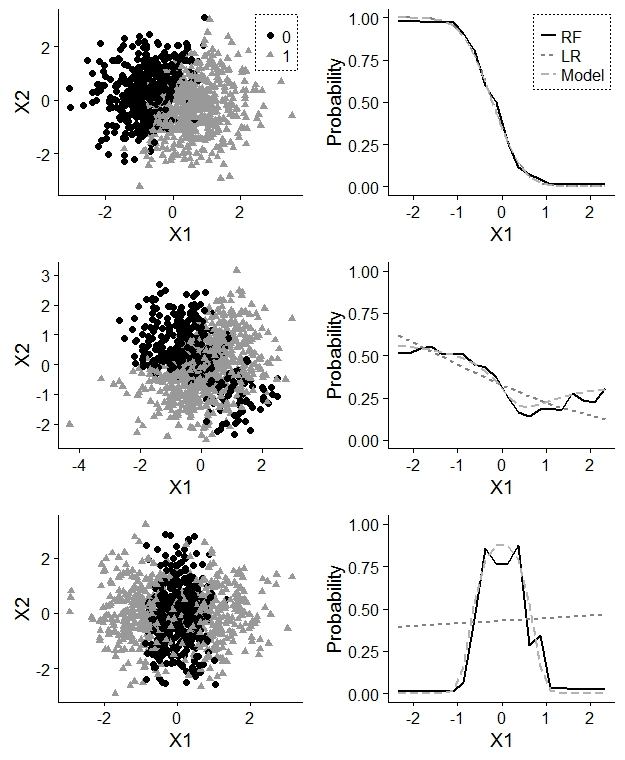
\includegraphics[width=12cm]{Images/PDP/PdpBlackWhite.jpeg}}
	\caption{Plot of the PDP for the tree simulated datasets. Each line is related to a dataset. On the left, visualization of the dataset. On the right, the partial dependance for the variable $X_1$. The datasets represent from top to bottom a linear, dependant, and non linear relation with the target.}
	\label{fig:plotPDP}
\end{figure}


\newpage
\subsection{Benchmarking with real data}
In this section we present the design of our benchmarking experiment. Most importantly, the experiment is based on a collection of $M$ real datasets (in contrast to other types of benchmarking experiments relying on simulated data). The prediction accuracy of LR and RF on real datasets is estimated through cross-validation as briefly presented in Section \ref{subsubsec:cv}. Issues related to the statistical analysis of the benchmarking results as discussed in Boulesteix et al. (The American Statistician 2015) are reviewed in Section \ref{subsubsec:stat}. 


\subsubsection{Cross-validation}
\label{subsubsec:cv}

In a $k$-fold cross-validation, the original sample is randomly split in $k$ subsamples of equal sizes. One of the fold is chosen as the test set, the k-1 others are used for training. The process is repeated $k$ times, and then the performances are averaged. We chose a 10 times 5-Cross Validation in our benchmark (the 5-CV is repeated 10 times), see \cite{Bischl2012} for advice on resampling methods. In the stratified version of the CV, the folds are chosen such that we have the same proportion of the classes in all the partitions. The stratified version was chosen because the proportion of imbalanced dataset was important. With too imbalanced datasets, it may happen that a level of a categorical feature is present in the test set, but not present in the train set, in which case the logistic regression cannot be applied. At the end we obtain results in the form of a $M\times 2$ data matrix containing the CV errors of LR (first column) and RF (second column) for the $M$ considered datasets.


\subsubsection{Accuracy measures}
Given a classifier, let $\hat{f}(i,j)$ represent the estimated probability of observation $i$ belonging to class $j$, $f(i,j)=1_{i∈j}$ the true probability of example $i$ to be of class $j$. $C(i,j) \in \{0,1\}$, it equals 1 if  $f(i,j)$ made the right prediction, else 0. $n$ is the number of observations of the dataset, and $c$ the number of classes. In our study, we consider the following measures quantifying prediction accuracy in the case of a binary classification problem \citep{ferri2009experimental}.

\begin{itemize}

\item The Accuracy, proportion of correct prediction:  
\\ $Acc =  \sum_{i=1}^N \sum_{j=1}^c f(i,j)C(i,j)$

\item The Area Under Curve, average of the error for each class: 
\\$Auc =  \frac{\sum_{i=1}^N f(i,j) \sum_{t=1}^n}{n_j n_k}   I(f(i,j)f(t,j))$


\item The Brier Score, which penalizes strong deviations from the true probability:
\\ $Brier =  \frac{\sum_{j=1}^c \sum_{i=1}^n (f(i,j)-\hat{f}(i,j))^2} {n}$


\end{itemize}

The time of training was also added.



\subsubsection{Statistical analysis}
\label{subsubsec:stat}
summary of Boulesteix et al. (The American Statistician 2015)
\textbf{???}

\subsubsection{The OpenML database}
\label{subsubsec:OpenML}

So far we have said that the benchmarking experiment used a collection of $M$ real datasets without specifying which ones. In practice, one often uses already formatted datasets from public databases for this purpose. Many of them offer a user-friendly interface and a good documentation which facilitate to some extent the preliminary steps of the benchmarking experiment (search for datasets, data download, preprocessing). One of the most well-known such databases is UCI repository, see \cite{Lichman:2013}. Specific scientific areas may have their own databases, such as ArrayExpress and GEO for molecular data from high-throughput experiments, see \cite{brazma2003arrayexpress} and  \cite{ncbiarchive} respectively. Most recently, the OpenML database \citep{vanschoren2014openml} has been initiated as an exchange platform allowing machine learning scientists to share their data and results. This database includes as many as 19625 datasets as of october 2016, a non-negligible proportion of which are relevant as example datasets for benchmarking classification methods.


\subsubsection{Inclusion criteria}
\label{subsubsec:incl}
When using a huge database of datasets, it becomes obvious that one has to define criteria for inclusion in the benchmarking experiment. Inclusion criteria in this context do not have any long tradition in computational science. The criteria used by researchers to select datasets are most often completely non-transparent. It is often the fact that they select a number of datasets which were found to somehow fit the scope of the investigated methods, but without clear definition of this scope. 

We conjecture that datasets are occasionally removed from the experiment {\it a posteriori} because the results do not meet the expectations/hopes of the researcher. While the vast majority of researchers certainly do not cheat consciously, such practices may substantially bias the conclusion of a benchmarking experiment; see for instance \cite{yousefi2010reporting} \textbf{is it the right one ? Yousefi et al. (Bioinformatics 2010)} for theoretical and empirical investigation of this problem. In a word, \lq\lq fishing for datasets'' should be prohibited, see Rule 4 of \cite{boulesteix2015ten}.

Even if fishing for datasets is prohibited, it is important that criteria for inclusion in the benchmarking experiment are clearly stated; \textbf{see Boulesteix, Wilson and Hapfelmeier (technical report 2016, coming soon)} for an extensive discussion of this issue.

In our study, we consider the following datasets' characteristics to define inclusion criteria:
\begin{itemize}
\item $n$: number of observations
\item $p$: number of features
\item	$\frac{p}{n}$ 
\item	$d$ : dimension of the dataset
\item	$\frac{d}{n}$ 
\item	$C_{min}$ Percentage of elements of the minority class
\item	$C_{max}$ Percentage of elements of the majority class
\item	$p_{numeric}$ : number of numeric features
\item	$p_{categorical}$ : number of categorical features
\item $timetrain$ : duration for the run a 5-fold CV with a default Random Forest 
\end{itemize}

Based on these datasets' characteristics, we define several sets of inclusion criteria and investigate the impact of this choice on the results of the benchmarking experiment. In the same vein, one can also analyse the results of benchmarking experiments for different subsets of datasets successively, following the principle of subgroup analyses performed in clinical trials. For example, one could analyse the results for \lq\lq large'' datasets ($n>1000$) and \lq\lq small datasets'' ($n\leq 1000$) separately.


\subsubsection{Meta-learning}
Going one step further, one can try to model the difference between the methods' performances based on the datasets' characteristics. Such a modelling approach can be seen as a simple form of {\it meta-learning}---a well-known task in machine learning.

\newpage

\section{Results}

We consider a set of $M$ datasets . Each one of its observations is a dataset from openML. For each observation we compute the performance of the different learners we consider: random forest, logistic regression and its penalized versions. Several packages are used: mlr for higher abstraction and a simpler way to compute benchmarks \citep{mlrpackage}, openML for loading the datasets \citep{openMLpackage}, and snowfall for parallel computing \citep{snowfallpackage}. We give more details on the parameters of the benchmark in the subsections.

\subsection{Datasets}
Details on the criteria for dataset selection are important. On the ~20000 datasets from OpenML, we select the binary classification problem. We remove the datasets that include missing values, the high dimentional datasets such that $p>n$, and the obvious simulated datasets to consider 240 datasets.

\begin{figure}[h]
	\centerline{
		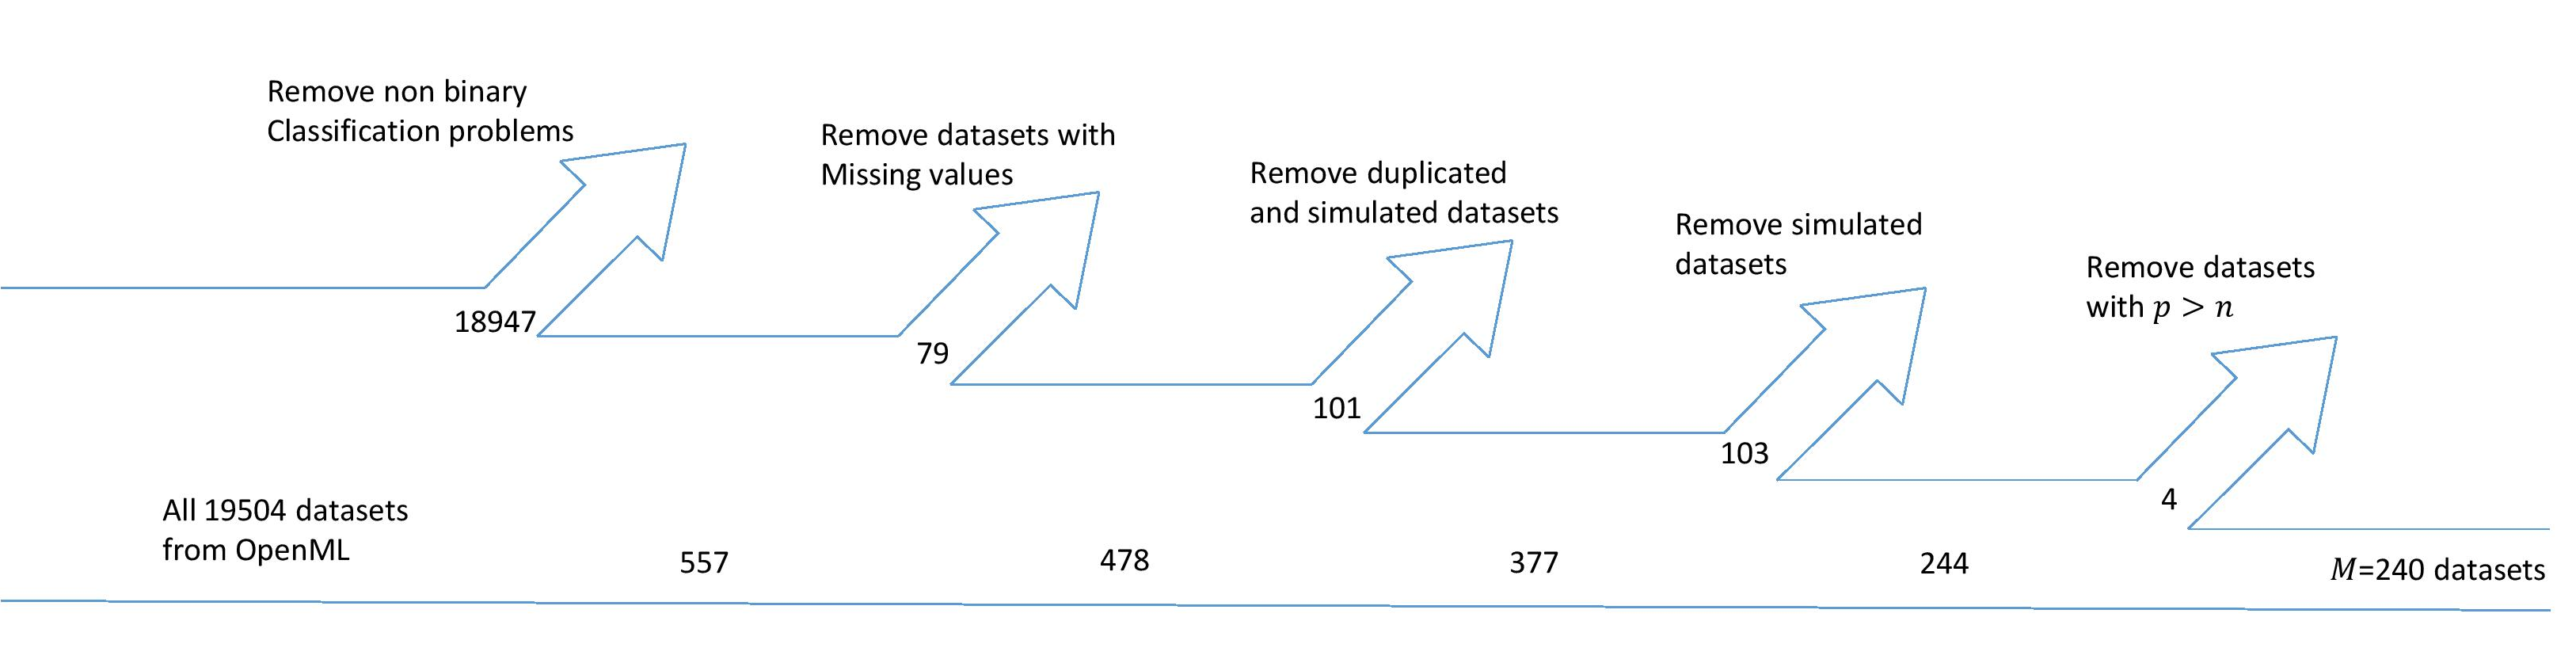
\includegraphics[width=14cm]{Schemas/FlowChart-paint.png}}
	\caption{Flowchart representing the criteria for selection of the datasets.}
	\label{fig:flowchartdataset}
\end{figure}

\textbf{Distribution of the datasets characteristics ?}

\newpage
\subsection{Overall results}


\begin{table}[h]
   \begin{tabular}{| c | c | c | c | c | c | c |}
     \hline
		  & $acc$ & $auc$ & $brier$ & $ber$ & $logloss$ & $timetrain$ \\ \hline
     Logistic regression & 0.825 & 0.830 & 0.129 & 0.235 & 1.169 & 0.152 \\ \hline
     Random forest & 0.853 & 0.869 & 0.103 & 0.211 & 0.374 & 3.133 \\ \hline
     %\hline
   \end{tabular}
	\quad
	   \begin{tabular}{| c | c | c | c | c | c | c |}
     \hline
		  & $acc$ & $auc$ & $brier$ & $ber$ & $logloss$ & $timetrain$ \\ \hline
     Logistic regression & 1.710 & 1.720 & 1.720 & 1.614 & 1.684 & 1.008 \\ \hline
     Random forest & 1.290 & 1.280 & 1.280 & 1.386 & 1.316 & 1.992 \\ \hline
     %\hline
   \end{tabular}
	\caption{Table representing the performances for both LR and RF. On the top, the mean performance values. On the bottom, the mean ranks.}
  \label{table:meanperfs}
\end{table}


Overall performances are presented in table \ref{table:meanperfs} for all the measures. For the following sections, we decide to focus on the accuracy, as correlation is high between the different performance measures, and the results similar. We observe in figure \ref{fig:OverallResults} the boxplots of performances of Random Forest and Logistic Regression. We also plotted the boxplot of the difference in accuracy, and observed that Random Forest does better in most of the cases (71 \% of our datasets), and when logistic regression outperforms random forest the difference is minimal. The Nemeyi's test



\begin{figure}[h]
\begin{subfigure}{.5\textwidth}
  \centering
  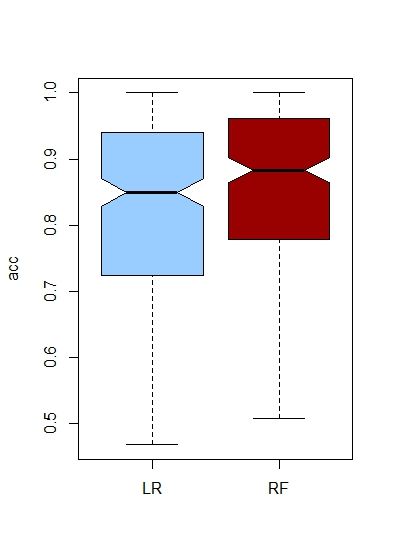
\includegraphics[width=.8\linewidth]{Images/Results/OverallGGplot.jpeg}

\end{subfigure}%
\begin{subfigure}{.5\textwidth}
  \centering
  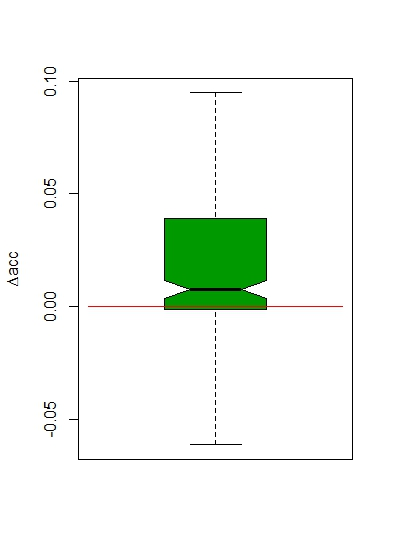
\includegraphics[width=.8\linewidth]{Images/Results/DiffAcc.jpeg}
\end{subfigure}
\caption{On the left, boxplot of the performance in accuracy for the random forest (in red) and the logistic regression (in blue). On the right, boxplot of the difference in accuracy between random forest and logistic regression. A red line is plotted at y=0.}
\label{fig:OverallResults}
\end{figure}



\newpage

\subsection{Explaining differences: datasets' characteristics}

\subsubsection{Principle}

While it is obvious to any computational scientist that the performance of methods may depend on some datasets' characteristics, this issue is not easy to investigate in real data settings because i) it requires a large number of datasets---a condition that is often not fulfilled in practice; ii) this problem is enhanced by the correlations between characteristics. In our benchmarking experiment, however, we consider such a huge number of datasets that an investigation of the relationship between methods' performances and datasets' characteristic becomes possible to some extent. We decide to illustrate this idea using only one dataset from OpenML in figure \ref{fig:DatasetDifferentp} with the datasets's feature $p^*$. For different values of $p$, $p \in \{1,p^*\}$ we randomly choose $N$ times $p$ features from our dataset to feed our algorithms and evaluate the performance. We observe in figure \ref{fig:DatasetDifferentp} that the accuracy increases for both logistic regression and random forest, as we expected. We also see that the accuracy of random forest increases faster than for logistic regression. Thus p seems like an important criteria when choosing between a random forest and a logistic regression.



\begin{figure}[h]
	\centerline{
		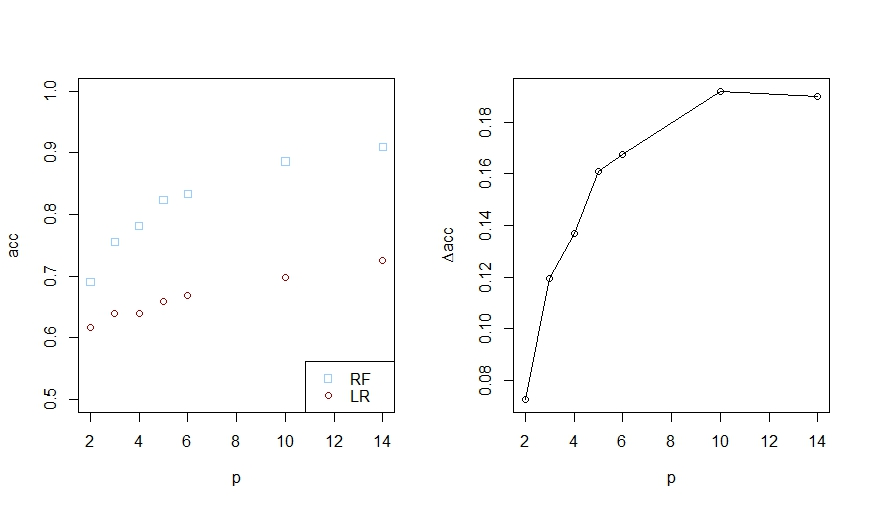
\includegraphics[width=12cm]{Images/Results/Dataset2p.jpeg}}
	\caption{On the left, mean evaluation of the performance of Rf and LR on the OpenML dataset (Id = 1496) for different values of $p$. On the left, plot of the difference of the mean performance $\Delta acc = acc_{RF}-acc_{LR}$. Here $p \in \{2,4,5,6,10,14\}$ and the performance is evaluated with a 2 times 5-CV.}
	\label{fig:DatasetDifferentp}
\end{figure}


\subsubsection{Results with varying inclusion criteria}
We decided to extend this idea, and studied the influence of the dataset's parameter on the difference in accuracy between random forest and logistic regression ($\Delta acc$). We computed the p-values of the Kendall and Spearman's test, and the significance value for the associated linear model. Results are shown in table \ref{table:correlation}. It seems the most relevant dataset's features are $p$ and its derivatives and $Brier_{LR}$.

\begin{table}[h]
   \begin{tabular}{| c | c | c | c |}
     \hline
		 & Spearman's $\rho$  p-value & Kendall's $\tau$ p-value & $\mathbb{P}(>|t|)$ \\ \hline
     $n$  & $3.52e^{-1}$ & $4.11e^{-1}$ &  $1.55e^{-1}$  \\ \hline
     $p$  & $1.35e^{-6}$  & $ 6.67e^{-7}$ & $3.10e^{-3}$  \\ \hline
     $\frac{p}{n}$  & $7.01e^{-2}$ & $9.67e^{-2}$ & $8.9e^{-1}$  \\ \hline
     $d$  & $5.50e^{-4}$ & $3.95e^{-4}$ &$ 4.30e^{-3}$  \\ \hline
     $\frac{d}{n}$ & $8.74e^{-2}$ & $1.42e^{-3}$ & $8.25e^{-1}$  \\ \hline
     $p_{numeric}$  & $2.78e{-4}$ & $1.56e{-4}$ & $2.89e{-1}$  \\ \hline
     $p_{categorical}$  & $1.73e{-1}$ & $1.64e{-1}$ & $4.10e{-3}$  \\ \hline
		 $p_{numeric,rate}$  & $5.87e{-4}$ & $2.96e{-4}$ & $6.27{-1}$  \\ \hline
     $p_{categorical,rate}$  & $5.87e{-4}$ & $2.96e{-4}$ & $6.27{-1}$  \\ \hline
     $C_{min}$ & $7.73e{-1}$ & $6.98{-1}$ & $6.87{-2}$  \\ \hline
     $C_{max}$ & $7.73e{-1}$ & $6.98{-1}$ & $6.87{-2}$  \\ \hline
     $Brier_{LR}$ & $5.35e{-4}$ & $3.16{-4}$ & $4.64{-8}$ \\ \hline

     %\hline
   \end{tabular}
	\caption{Table representing the correlation between $\Delta acc$ and the corresponding dataset's features.}
  \label{table:correlation}
\end{table}

We decide to 

\begin{figure}[h]
\begin{subfigure}{0.8\textwidth}
  \centering
  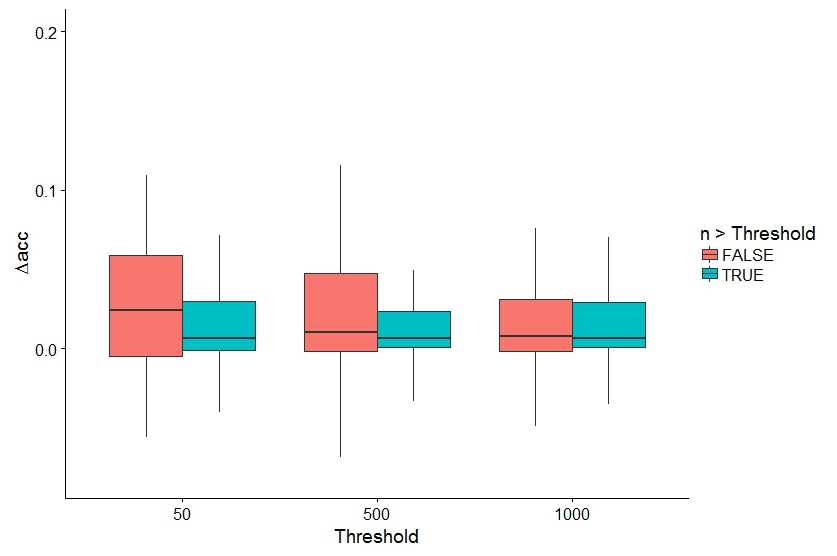
\includegraphics[width=.8\linewidth]{Images/Boxplots/boxplotn.jpeg}
\end{subfigure}%

\begin{subfigure}{0.8\textwidth}
  \centering
  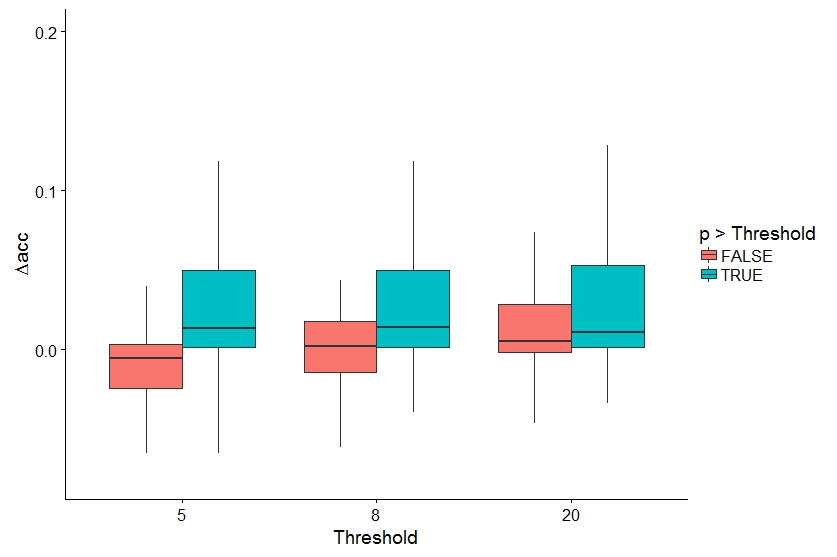
\includegraphics[width=.8\linewidth]{Images/Boxplots/boxplotp.jpeg}
\end{subfigure}

\begin{subfigure}{0.8\textwidth}
  \centering
  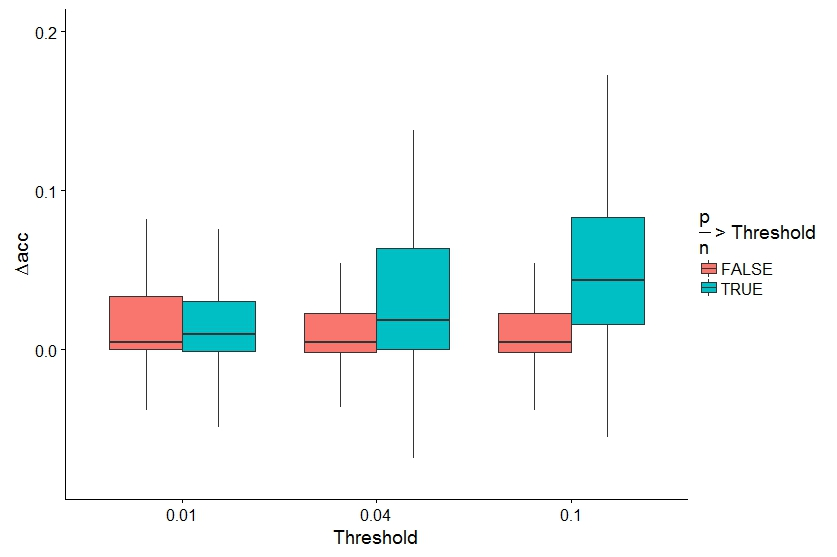
\includegraphics[width=.8\linewidth]{Images/Boxplots/boxplotpsurn.jpeg}
\end{subfigure}

\caption{Boxplots of $\Delta acc$ for different threshold as criteria for dataset's selection. On the top, boxplots for feature $n$, on the middle for feature $p$ and on the bottom for the feature $\frac{p}{n}$.  }
\label{fig:Boxplots}
\end{figure}



\subsubsection{Subgroup analysis as additional file?  \textbf{?? I don't understand this part ??}}

\subsubsection{Meta-learning}

Do a Cart Tree and see ??? How much performance ?



\subsection{Explaining differences: partial dependence plots}
\begin{itemize}
\item In the previous section we have investigated the impact of datasets' characteristics on the results of benchmarking and simply modeled the difference between methods' performance based on these characteristics. 
\item In this section, we take a different approach to the explanation of differences. We use partial dependence plots as a technique to assess the dependency pattern between response and predictors underlying the prediction rule. When the methods' performances are different, we intuitively expect these dependency patterns to be different, sampling variations put aside. We typically expect this to be the case when the true joint distribution of response and predictors is far from the logistic regression model or when the logistic regression model holds but RF fails to recover it (due to, e.g., too small sample size). 
\item 
\end{itemize}

\newpage
\section{Test Bibliography}

\bibliography{bibli}

\end{document}

